\section{入力の設計方法}
離散時間線形時不変システム
\begin{align}
    \label{state2}
    x_{t+1} &= Ax_t + Bu_t + w_t \\
    \label{output2}
    y_t &= Cx_t + Du_t + z_t
\end{align}
を考える.ただし,
$x_t \in \mathbb{R}^n,u_t \in \mathbb{R}^p,y_t \in \mathbb{R}^m$はそれぞれ時刻$t$におけるシステムの状態,入力,出力を表す.また,$w_t \in \mathbb{R}^n,z_t \in \mathbb{R}^m$はプロセスノイズおよび観測ノイズを表し,$w_t \sim \mathcal{N}(0, \sigma_w^2I), z_t \sim \mathcal{N}(0, \sigma_z^2I)$である.
初期状態$x_1 = 0$であり,$\rho(A) \leq \eta <1$と仮定する.ここで,$\rho(\cdot)$は行列の最大固有値の絶対値を表す.
また,入力に関する制約条件
\begin{align*}
    |u_{tk}| \leq a,  \quad (\forall t = 1, 2, \ldots,\quad  k = 1, 2, \ldots,p) 
\end{align*}
を加える.ここで,$a$は既知の正の実数である.

2.3節の手順に従い,$G$の最小二乗推定を行う.
$G$の最小二乗推定値の推定誤差のスペクトルノルムの上界は(\ref{error})式より,
\begin{align}
    \| \hat{G} - G \| &= \| (U^*U)^{-1}U^* (W \cdot F +E + Z) \| \notag\\
    \label{error_norm}
    &\leq \| (U^*U)^{-1}U^* \| (\|W\| \cdot \|F\| +\|E\| + \|Z\|) 
\end{align}
となる.\eqref{error_norm}式の右辺を最小化するための入力設計を考える.入力の項について,
\begin{align*}
    \| (U^*U)^{-1}U^* \|^2 &= \lambda_{\max}\{((U^*U)^{-1}U^*)((U^*U)^{-1}U^*)^* \}
    \\
    &=\lambda_{\max}((U^*U)^{-1} )
    \\
    &= \frac{1}{\lambda_{\min}(U^*U)}
    \\
    &= \frac{1}{\sigma_{\min}^2(U)}
\end{align*}
が成り立つ.ここで$\lambda_{\min}(\cdot), \lambda_{\mathrm{max}}(\cdot)$は,それぞれ行列の最小固有値,最大固有値を表し,$\sigma_{\min}(\cdot)$は行列の最小特異値を表す.
したがって推定誤差は,
\begin{equation}
    \| \hat{G} - G \| \leq \| \frac{|W\| \cdot \|F\| +\|E\| + \|Z\|}{\sigma_{\min}(U)}
\end{equation}
である.

したがって$\sigma_{\text{min}}(U)$を大きくすると,推定誤差のノルムがより小さくすることができる.
入力信号の大きさに上界を与えて以下の問題を考える.\\
\par
\textbf{問題1:}
\begin{align*}
    & \text{maximize} &&  \sigma_{\min}(U) 
    \\
    & \text{subject to} 
    && |u_{tk}| \leq a &t &= 1, 2, \ldots,\bar{N}, \\
    &&&&k &= 1, 2, \ldots,p 
\end{align*}

この入力を決定する問題は凸問題ではないため,解くことは容易ではない.
そこで,この問題の最適値に近い値をとる入力を設計するために,以下の補題を用いる.


\begin{sub}
\cite{RAFA}
\label{sub_input_alg}
与えた$\delta \in (0, 1)$, $\epsilon \in (0, 1)$について,
\begin{equation*}
    M \geq \frac{\log{\frac{1}{\delta}}}{\log\frac{1}{1-\epsilon}}
\end{equation*}
を満たすサンプル数$M$を考える.  
入力をある確率分布に従って$M$回生成し,それらを
\eqref{U}式の$U$に従いならべ,
\begin{equation*}
    \{ U^{(i)}, 1 \leq i \leq M \} 
\end{equation*}
とする.このとき$U$の最小特異値
\begin{equation*}
    \{\sigma_{\min}(U^{(i)}),  1 \leq i \leq M\}
\end{equation*}
の最大値
\begin{equation*}
    \hat{\gamma}_M = \underset{i = 1, \ldots, M}{\max}\sigma_{\min}(U^{(i)})
\end{equation*}
は,$1-\delta$以上の確率で
\begin{equation}
    \mathbb{P} \{ \sigma_{\min}(U) \leq \hat{\gamma}_M \} \geq 1-\epsilon
\end{equation}
を満たす.
\end{sub}

\section{入力を生成する確率分布の検討}
% $T, \bar{N}$を大きくした場合について,
補題\ref{sub_input_alg}に基づき,どの確率分布を選択してアルゴリズムを適用すれば問題1の最適値により近い入力が得られるかを数値実験により検証する.



$m = 1, p = 1, n = 2$として,システムの行列を
\begin{align*}
    A &= 
    \begin{bmatrix}
        0.6 & 0.1 \\
        0.2 & 0.4
    \end{bmatrix},
    B =
    \begin{bmatrix}
        1 \\
        1
    \end{bmatrix},
        C =
    \begin{bmatrix}
        1 & 1 
    \end{bmatrix}, 
    D = 1
\end{align*}
と設定する.行列$A$の固有値は,
\begin{align*}
    \lambda_1 = \frac{-\sqrt{3}+5}{10}, \quad \lambda_2 = \frac{\sqrt{3}+5}{10}
\end{align*}
であり,$\lambda_1, \lambda_2 <1$より,安定なシステムである.
プロセスノイズ,観測ノイズについて,$\sigma_w = \sigma_z = 0.5$とする.
推定するマルコフパラメータの長さについては$T = 20$として,学習回数を$N = 1000$までとり,50刻みで推定誤差についてプロットした.
各分布に対して,補題\ref{sub_input_alg}を用いて設計した入力について$G$の最小二乗推定値を計算し,真値との推定誤差を10回出力し,その平均についてプロットしている.

\begin{figure}[htbp]
    \centering
    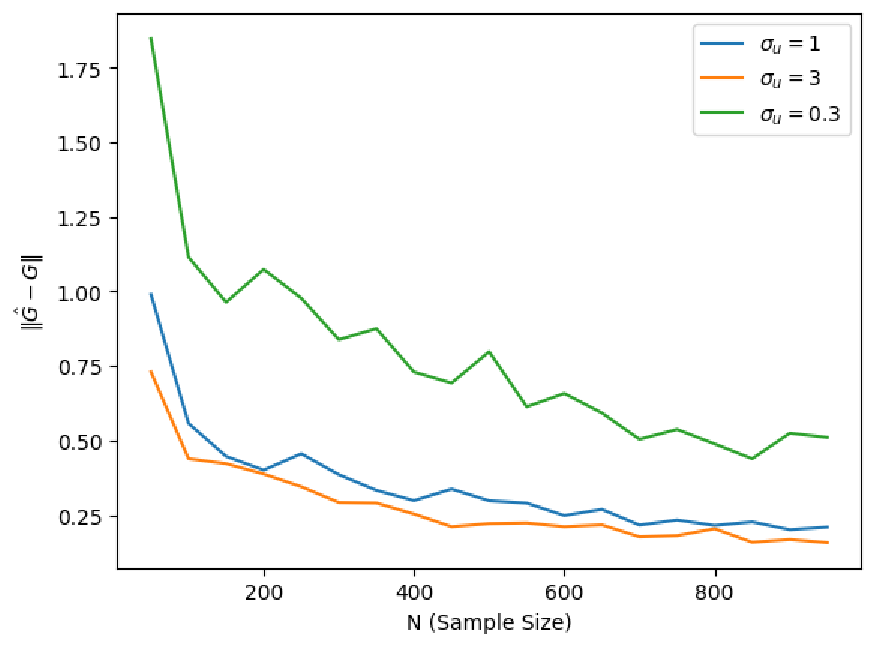
\includegraphics[width=0.8\linewidth]{figure/figure1.pdf}
    \caption{正規分布の分散を変えたときの比較}
    \label{sigma_change}
\end{figure}

図\ref{sigma_change}は,補題\ref{sub_input_alg}を用いる際に,正規分布に従う入力を選択した場合における分散の違いが推定精度に与える影響を比較したものである.


この図から,推定精度は分散の大きさ依存していることが分かる.
入力の制約は,
\begin{equation*}
|u_{t}| \leq 1, \quad \quad  t = 1, 2, \ldots,\bar{N}
\end{equation*}
とした.そのため
正規分布$\mathcal{N}(0, \sigma_u^2)$に従う確率変数$X$ついて,$X>1$のとき$X = 1$,$X<-1$のとき$X = -1$としている.
この分布を丸めた正規分布と呼ぶ.

図\ref{t_vs_c}では,$\mathcal{N}(0, 1)$を丸めた正規分布(clipped normal distribution)と切断正規分布(truncated normal distribution)を比較している.
切断正規分布とは,通常の正規分布を$-a \leq x \leq b$の範囲に制限した分布である.確率密度関数は
\begin{equation*}
f(x|\mu, \sigma, a, b) =
\begin{cases}
0, & \text{if } x \leq a, \\
\frac{\phi(\frac{x-\mu}{\sigma})}{\Phi(\frac{b-\mu}{\sigma}) - \Phi(\frac{a-\mu}{\sigma})}, & \text{if } a < x < b, \\
0, & \text{if } b \leq x.
\end{cases}
\end{equation*}
と表される.ここで$\phi(z), \Phi(z)$はそれぞれ標準正規分布$\mathcal{N}(0, 1)$の確率密度関数,累積分布関数を表しており,
\begin{align*}
    \phi(z) = \frac{1}{\sqrt{2\pi}}e^{-\frac{z^2}{2}}, \quad
    \Phi(z) = \int_{-\infty}^{z} \phi(t) \, dt
\end{align*}
である.
\begin{figure}[htbp]
    \centering
    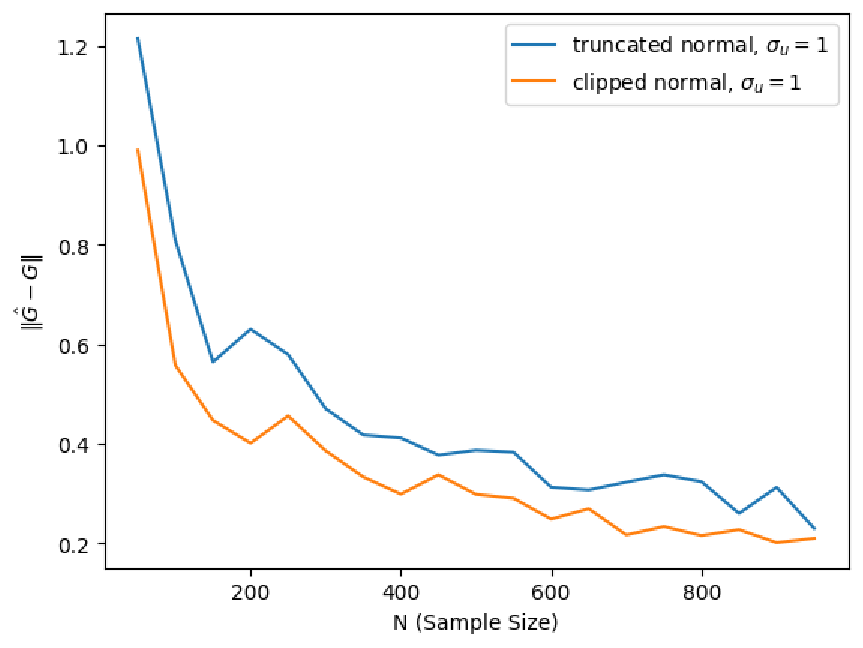
\includegraphics[width=0.8\linewidth]{figure/figure2.pdf}
    \caption{切断正規分布と丸めた正規分布の比較}
    \label{t_vs_c}
\end{figure}
図\ref{t_vs_c}において,切断正規分布は$\mathcal{N}(0, 1)$を$[-1, 1]$で制限している.
丸めた正規分布と切断正規分布を比較すると,丸めた正規分布の方が推定精度が高いことがわかる.

図\ref{u_vs_n_vs_b}では,$\mathcal{N}(0, 1)$を丸めた正規分布と一様分布$\mathcal{U}[-1, 1]$,$\{-1, +1\}$を等確率でとるベルヌーイ試行の3つの分布について比較している.
\begin{figure}[htbp]
    \centering
    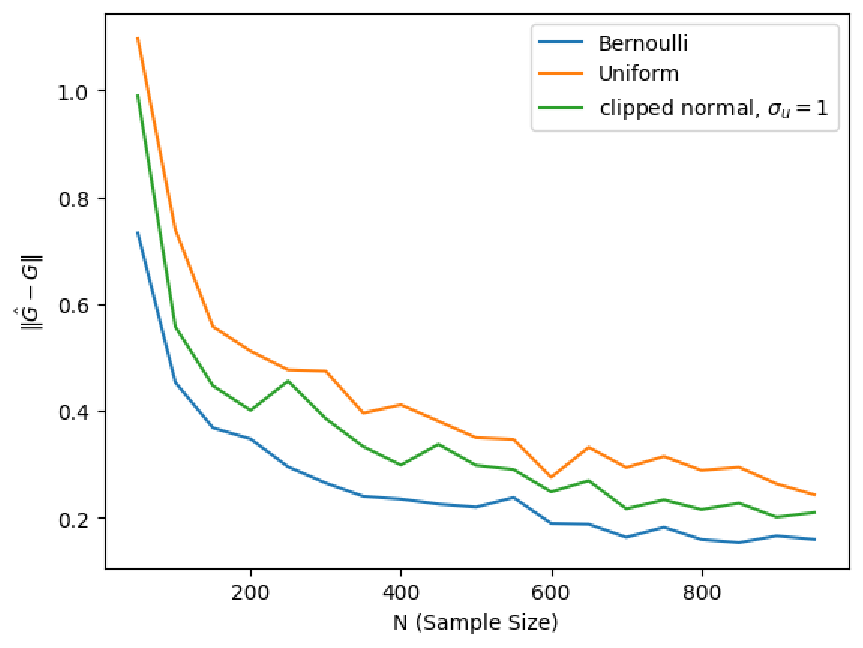
\includegraphics[width=0.8\linewidth]{figure/figure3.pdf}
    \caption{一様分布,ベルヌーイ分布,正規分布の比較}
    \label{u_vs_n_vs_b}
\end{figure}

次の図\ref{x^n}では,
\begin{equation*}
    y = \frac{2k+1}{2}x^{2k}, \quad (-1 \leq x\leq 1)
\end{equation*}
の確率分布と,ベルヌーイ試行について推定誤差を比較している.この分布は$k \to \infty$で$\{-1,+1\}$を等確率でとるベルヌーイ試行に収束する.
$k = 1, 2$の場合である
$f(x) = \frac{3}{2}x^2, f(x) = \frac{5}{2}x^4$と$\{-1, +1\}$を等確率でとるベルヌーイ試行を比較した.

\begin{figure}[htbp]
    \centering
    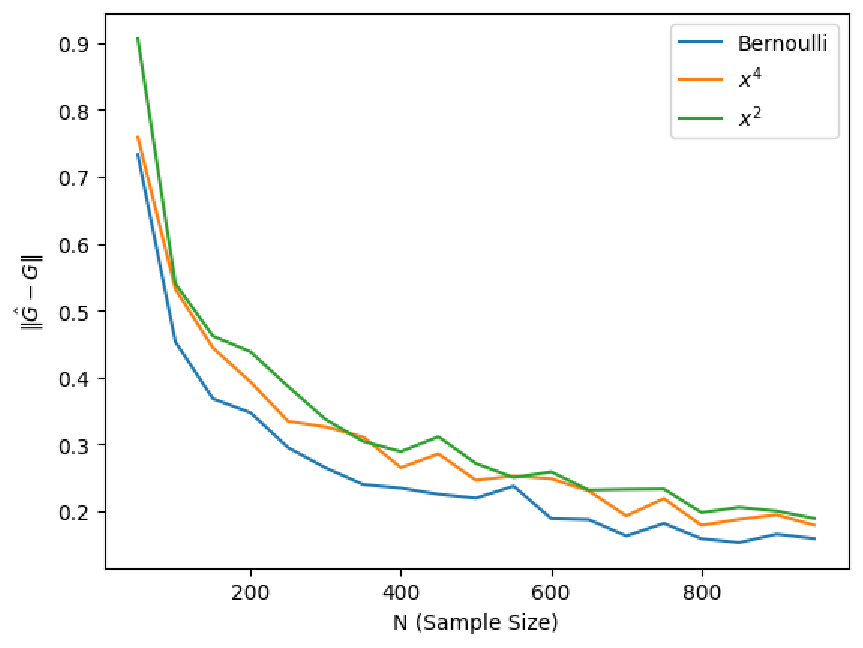
\includegraphics[width=0.8\linewidth]{figure/figure4.pdf}
    \caption{$f(x) = \frac{3}{2}x^2, f(x) = \frac{5}{2}x^4$, ベルヌーイ分布の比較}
    \label{x^n}
\end{figure}

以上の比較から,$\{-1, +1\}$に近い値を高確率でとる分布が推定誤差を小さくしていることがわかる.
\\
実際に$T, N$を固定した低次元の場合について,問題1を解いた場合の結果を以下に示す.
入力の次元は,$p=1$として,各時刻の入力に対し,$|u_t| \leq 1,  (t = 1, 2, \ldots , \bar{N})$とした.
$T = 4, \bar{N} = 7$の場合について,問題1の最適解の1つは,
\begin{equation*}
    U = 
    \begin{bmatrix}
    1 & 1 & -1 & 1 \\
    -1 & 1 & 1 & -1 \\
    1 & 1 & 1 & 1 \\
    1 & -1 & 1 & 1
    \end{bmatrix}
\end{equation*}
であり,最適値は$\sigma_{\text{min}}(U) = 2$である.

また,$T = 4, \bar{N} = 8$の場合について,問題1の最適解の1つは,
\begin{equation*}
    U = 
    \begin{bmatrix}
    1 & 1 & -1 & 1  \\
    1 & 1 & 1 & -1 \\
    1 & 1 & 1 & 1  \\
    -1 & 1 & 1 & 1 \\
    1 & -1 & 1 & 1
    \end{bmatrix}
\end{equation*}
であり,最適値は$\sigma_{\text{min}}(U) = 2$である.
この結果からも$\{-1, +1\}$を等確率でとる分布を選択するのが良いことが分かる.\\

実際に,補題\ref{sub_input_alg}のアルゴリズムに対して,$\{-1, +1\}$を等確率でとる確率変数を用いて入力を設計し,その入力に基づいて得られた最小二乗推定値と,先行研究の入力が正規分布に従い生成される場合の最小二乗推定値を比較した.
用いたサンプル数は,$N = 100$で,$\epsilon = \delta = 0.0001$としたときに補題\ref{sub_input_alg}を満たす$M$として,$M = 100000$とした.表~\ref{table_1}から,入力に制約のない場合よりも推定精度が高いことがわかる.

\begin{table}[h!]
\caption{入力をマルコフパラメータの最小二乗推定値}
\centering
\begin{tabular}{l|rrrr}
                    & $D$      & $CB$     & $CAB$  & $CA^2B$     \\ \hline \hline 
真値                 & 1      & 2      & 1.3 & 0.86 \\ \hline
$\mathcal{N}(0, 1)$ & 1.0923 & 2.0340 & 1.4414  & 0.9217 \\ \hline
提案手法              & 1.0443 & 2.0321 & 1.3640  & 0.8664                   
\end{tabular}
\label{table_1}
\end{table}

\section{推定誤差の上界}
入力を設計した場合の行列$G$の最小二乗推定値と真値の誤差のスペクトルノルムの上界について,以下の定理を示す.

\begin{thm}
$\bar{N} = N + T - 1 $時間の入出力データが与えられたとき,任意の$\delta \in (0, 1)$について$G$の最小二乗推定値$\hat{G}$について,$1- 3\delta$以上の確率で
\begin{align}
\label{upper_bound}
    \|\hat{G}-G\| &\leq \frac{R_w\|F\| +R_e + R_z}{\sigma_{\mathrm{min}}(U)}
\end{align}
が成立する.ただし,
\begin{align*}
    R_w &= \sigma_w\sqrt{ 2\max\{N, pT\}\log{\left(\frac{N+pT}{\delta}\right)}}
    \\
    R_e &=\|C\|\eta^{T-1} \sum_{t = T}^{\bar{N}}\sum_{i = 1}^{t-T-i}\eta^{t-T-i}\|Bu_i\| \\ 
    &\quad + N\frac{\sigma_w\eta^{T-1}}{\sqrt{1-\eta^2}} \|C\| \sqrt{m + \sqrt{8m\log{(2/\delta)}}}
    \\
    R_z &= \sigma_z(\sqrt{N} + \sqrt{m}+ \sqrt{\log{1/\delta}})
\end{align*}
である.
\end{thm}

\begin{proof}
% \textbf{証明: }
まず,ノイズの項$\|Z\|$の上界を与える.
付録Aの補題\ref{Z_bound}より,$1-\delta$以上の確率で
\begin{equation*}
    \|Z\| \leq \sigma_z(\sqrt{N} + \sqrt{m} + \sqrt{\log{1/  \delta}} )
\end{equation*}
が成り立つ.

次に,$\|W\|$の上界を与える.まず,$w_t$がスカラーである場合$(p = 1)$を考える.
\begin{align*}
    W^* &= 
    \begin{bmatrix}
        W_T     & W_{T+1} & \cdots & W_{\bar{N}} \\
        W_{T-1} & W_T     & \cdots & W_{\bar{N}-1} \\
        \vdots  & \vdots  & \ddots & \cdots \\
        W_1     & W_2     & \cdots & W_N
    \end{bmatrix}\in\mathbb{R}^{T \times N} 
\end{align*}
であるから,
\begin{align*}
    B_1 = 
    \begin{bmatrix}
        0 & 0 &\cdots & 0 \\
        0 & 0 &\cdots & 0 \\
        \vdots & \vdots & \ddots &\vdots\\
        1 & 0 & \cdots & 0
    \end{bmatrix}
    , B_2 = 
    \begin{bmatrix}
        0 & 0 &\cdots & 0 \\
        \vdots & \vdots &\ddots & 0 \\
        1 & 0 & \ddots &\vdots\\
        0 & 1 & \cdots & 0
    \end{bmatrix}, \cdots, B_{\bar{N}} = 
    \begin{bmatrix}
        0 & 0 &\cdots & 1 \\
        0 & 0 &\cdots & 0 \\
        \vdots & \vdots & \ddots &\vdots\\
        0 & 0 & \cdots & 0   
    \end{bmatrix}
\end{align*}
と定義すると,
\begin{align*}
    W^* = w_1B_1 + w_2B_2 + \cdots + w_{\bar{N}}B_{\bar{N}} 
\end{align*}
と表すことができる.ここで,
補題\ref{W_bound}から,Wの分散に関する統計量$v(W)$を,
\begin{align*}
    v(W) &= \sigma_w^2\max \left\{ \sum_{k}B_kB_k^*, \sum_{k}B_k^*B_k \right\} \\
    &=\sigma_w^2 \max\{NI, TI\} \\
    &=\sigma_w^2 \max\{N, T\}
\end{align*}
とする.
$w_t \sim \mathcal{N}(0, \sigma_w^2I)$であるから,$w_t$がベクトル$(p >1)$の場合も同様に考えることができ,このとき
$v(W) = \sigma_w^2 \max\{N, pT\}$であるから,
\begin{equation*}
    \mathbb{P}\{ \|W\| \geq t\} \leq \exp{\left(\frac{-t^2}{2\sigma_w^2 \max\{N, pT\}}\right)} 
\end{equation*}
$\exp{\left(\frac{-t^2}{2\sigma_w^2 \max\{N, pT\}}\right)}=\delta$とおき,$\delta$について解くと,
\begin{equation*}
\label{W}
    \mathbb{P} \left\{ \|W\| \leq \sigma_w\sqrt{ 2\max\{N, pT\}\log{\left(\frac{N+pT}{\delta}\right)} }\right\} \geq 1-\delta
\end{equation*}
が成り立つ.

次に,$\|E\|$の項の上界について考える.
\begin{align*}
    e_t &= CA^{T-1}x_{t-T+1} \\
    &= CA^{T-1} 
    \begin{bmatrix}
        B & AB & \ldots & A^{t-T-1}B
    \end{bmatrix}
    \begin{bmatrix}
        u_{t-T}\\
        \vdots\\
        u_1
    \end{bmatrix}\\
    &\quad+ CA^{T-1}
        \begin{bmatrix}
        I & A & \ldots & A^{t-T-1}
    \end{bmatrix}
    \begin{bmatrix}
        w_{t-T}\\
        \vdots\\
        w_1
    \end{bmatrix}
\end{align*}
と展開できる.

\begin{equation*}
    W_t = CA^{T-1} \sum_{i = 0}^{t-T-1}A^iw_{t-T-i}
\end{equation*}
とすると,$e_t$の共分散行列は$\mathbb{E}[W_tW_t^*]$で表されるので,$w_t \sim \mathcal{N}(0, \sigma_w^2I)$であることから,
\begin{align*}
    X_t &= CA^{T-1} \sum_{i = 1}^{t-T} A^{t-T-i}Bu_i\\
    \Sigma(e_t) &=\mathbb{E}[W_tW_t^*] \\
    &= CA^{T-1} \left\{ \sum_{i = 0}^{t-T-1} \sigma_w^2 A^i(A^*)^i \right\}(A^{T-1})^*C^*
\end{align*}
とすると,$e_t$は,$\mathcal{N}(X_t, \Sigma(e_t))$に従う.
また
$\rho(A) \leq \eta$
であるから,
\begin{align*}
    \Sigma(e_t) &\leq CA^{T-1} \left\{ \sum_{i = 0}^\infty \sigma_w^2 A^i(A^*)^i \right\}({A^{T-1}})^*C^*\\
    &\leq \frac{\sigma_w^2\eta^{2(T-1)}}{1-\eta^2}CC^*\\
    & = \Sigma_e
\end{align*}
とすると上界を導出するにあたって,
$e_t \sim \mathcal{N}(X_t, \Sigma_e)$
と見積もってもよい.したがって,
$\tilde{e}_t = (\Sigma_e)^{-1/2}(e_t-X_t)$
は
$\mathcal{N}(0, I_n)$
に従う.これを$e_t$について解くと,
$e_t = (\Sigma_e)^{1/2}(\tilde{e_t})+X_t$
となるので,
\begin{align*}
    \|e_t\| &= \| (\Sigma_e)^{1/2}  \tilde{e}_t  + X_t\| \\
    &\leq \| \Sigma_e \|^{1/2} \| \tilde{e}_t \| + \|X_t\|
\end{align*}
が成り立つ.したがって,\eqref{E}式より,
\begin{align*}
    \|E\| &\leq \|e_T\| + \|e_{T+1}\| + \cdots + \|e_{\bar{N}}\| \\
    &\leq N \| \Sigma_e \|^{1/2} \| \tilde{e}_t \|  +\sum_{t = T}^{\bar{N}}\|X_t\| 
\end{align*}
が成り立つ.ここで,
\begin{align*}
    \sum_{t = T}^{\bar{N}}\|X_t\| &= \sum_{t = T}^{\bar{N}}\|CA^{T-1} \sum_{i = 1}^{t-T}A^{t-T-i}Bu_i\| \\
    &\leq \|C\|\eta^{T-1} \sum_{t = T}^{\bar{N}}\sum_{i = 1}^{t-T}\eta^{t-T-i}\|Bu_i\|
\end{align*}
である.

また,$\|\tilde{e}_t\|^2$は自由度$m$の$\chi$二乗分布に従うので,付録Aの補題\ref{chi^2_bound}より,
\begin{align*}
    \mathbb{P}\left[\left|\frac{1}{m}\|\tilde{e}_t\|^2 -1 \right| \geq t \right] \leq 2e^{-nt^2/8}
\end{align*}
が成り立つ.右辺を$\delta$として整理すると,
$1-\delta$以上の確率で
\begin{equation*}
    \|\tilde{e}_t\| \leq \sqrt{m + \sqrt{8m\log{(2/\delta)}}}
\end{equation*}
が成り立つことが分かる.

以上を組み合わせると$G$の推定誤差の上界\eqref{upper_bound}式が得られる.
\end{proof}

また,今回の問題設定では入力の大きさに上界$|u_{tk}| \leq a,  \quad (\forall t = 1, 2, \ldots,\quad  k = 1, 2, \ldots,p)$を課している.付録Bから,上界,下界のある確率分布から入力を設計しているため,設計した入力はsub-Gaussian性を持つことが分かる.
2章で紹介した定理\ref{thm_prev_error_bound}は,入力がsub-Gaussian性を持つ確率分布から生成されていれば用いることができる.

正規分布$\mathcal{N}(\mu, \sigma^2)$はに従う変数$X$は,パラメータ$\sigma$のsub-Gaussianである.
また,補題\ref{sub_input_alg}を用いて入力を設計する際に選択した$\{-a, +a\}$を等確率でとる確率分布から生成される確率変数も,例\ref{rad_ex}から,パラメータ$a$のsub-Gaussianであることが分かる.したがって,定理\ref{thm_prev_error_bound}や,補題\ref{sub_estimate_y}において入力の分散である$\sigma_u$をsub-Gaussianのパラメータに置き換えて考えることができる.十分大きな$N$における推定誤差の上界について,以下の定理を示す.

\begin{thm}
% \cite[Theorem3.2]{RHKB}
% \cite{RHKB}
\label{thm_prev_error_bound_2}
    $c, C >0$は十分大きな定数である.
    $\rho(A) < 1$であり,$\frac{N}{\log^2{(Np)}} \geq cpT\log^2{(pT)}$であるとする.
    $q = p+n$,$N_w = cTq\log^2{Tq}\log^2{Nq}$とする.
    また,入力がパラメータ$\sigma$の$\mathrm{sub-Gaussian}$である確率変数に従い生成されるとする.
    このとき,高い確率でマルコフパラメータ行列$G$の最小二乗推定値$\hat{G}$について,
    \begin{equation*}
        \| \hat{G}-G \| \leq \frac{R_w\|F\| + R_z + R_e}{\sigma\sqrt{N}}
    \end{equation*}
    が成り立つ.ここで,
    \begin{align*}
        R_z &= 8\sigma_z \sqrt{Tp + m} \\
        R_w &= \sigma_w (\sqrt{N_w} + N_w/\sqrt{N}) \\
        R_e &= C\sigma_e \sqrt{ \left( 1+\frac{mT}{N(1-\rho(A)^{T/2})}  \right)(Tp + m) }
    \end{align*}
    である.また,
    \begin{align*}
        \Phi(A) &= \sup_{\tau \geq 0} \frac{\|A^{\tau}\|}{\rho(A)^{\tau/2}} \\
        \Gamma_{\infty} &= \sum_{i = 0}^{\infty} \sigma_w^2A^i(A^*)^i + \sigma^2  A^iBB^*(A^*)^i
    \end{align*}
    とすると,
    \begin{equation*}
        \sigma_e = \Phi(A)\|CA^{T-1}\|\sqrt{\frac{T\|\Gamma_{\infty}\|}{1-\rho(A)^T}}
    \end{equation*}
    である.
\end{thm}